%% 由 build/emit_tex.py 生成（生成物，勿手改）；定制请放 user_style.tex / user_meta.yaml
\chapter{第 2 章 ·
解析函数}\label{ux7b2c-2-ux7ae0-ux89e3ux6790ux51fdux6570}

\section{§2.1
复变函数的概念、极限与连续性}\label{ux590dux53d8ux51fdux6570ux7684ux6982ux5ff5ux6781ux9650ux4e0eux8fdeux7eedux6027}

\begin{quote}
\textbf{本节目标}：掌握复变函数的概念、几何意义（映射）、反函数；理解复变函数极限的
\(\varepsilon\)-\(\delta\)
定义及其与二元实函数极限的联系；掌握复变函数连续的概念与判定。
\textbf{本节重点}：复变函数作为两个复平面上点集间的映射；极限与连续的概念；用实部/虚部函数研究极限与连续性。
\textbf{本节难点}：极限存在的充要条件（与二元实函数极限的等价性）；\(\arg z\)
的连续性（负实轴上的间断）。
\end{quote}

\subsection{2.1.1
复变函数的概念}\label{ux590dux53d8ux51fdux6570ux7684ux6982ux5ff5}

\textbf{定义 2.1} 设 \(E\) 为一复数集。若对 \(E\) 中每一个复数
\(z=x+iy\)，按照某种法则 \(f\) 有确定的一个或几个复数 \(w=u+iv\)
与之对应，那么称复变数 \(w\) 是复变数 \(z\)
的函数（简称\textbf{复变函数}），记作

\[
w=f(z).
\]

通常也称 \(w=f(z)\) 为定义在 \(E\) 上的复变函数，其中 \(E\)
称为\textbf{定义域}，\(E\) 中所有 \(z\) 对应的一切 \(w\)
值构成的集合称为 \(f(z)\) 的\textbf{值域}，记作 \(f(E)\) 或 \(G\)。

\begin{itemize}
\tightlist
\item
  若 \(z\) 的一个值对应着 \(w\) 的一个值，则称复变函数 \(f(z)\)
  是\textbf{单值}的；
\item
  若 \(z\) 的一个值对应着 \(w\) 的两个或两个以上的值，则称复变函数
  \(f(z)\) 是\textbf{多值}的。
\end{itemize}

\subsubsection{实部与虚部}\label{ux5b9eux90e8ux4e0eux865aux90e8}

复数 \(z=x+iy\) 与 \(w=u+iv\) 分别对应实数对 \((x,y)\) 和
\((u,v)\)。对于函数 \(w=f(z)\)，\(u\)、\(v\) 为 \(x\)、\(y\)
的二元实函数 \(u(x,y)\) 和 \(v(x,y)\)，所以 \(w=f(z)\) 又常写成

\[
w=f(z)=u(x,y)+iv(x,y).
\]

\textbf{例（\(w=z^2+1\)）} 令 \(z=x+iy\)，\(w=u+iv\)，那么

\[
w=u+iv=(x+iy)^2+1=x^2-y^2+1+2xyi,
\]

\(w=z^2+1\) 对应于两个实函数

\[
u=x^2-y^2+1,\qquad v=2xy.
\]

\subsubsection{复变函数的映射（几何）意义}\label{ux590dux53d8ux51fdux6570ux7684ux6620ux5c04ux51e0ux4f55ux610fux4e49}

对于复变函数 \(w=f(z)\) 即
\(u+iv=f(x+iy)\)，可以理解为两个复平面上的点集之间的映射。具体地说，复变函数
\(w=f(z)\) 给出了 \(z\) 平面上的点集 \(E\) 到 \(w\) 平面上的点集
\(f(E)\)（或 \(G\)）之间的一个对应关系：

\[
\forall z\in E \rightarrow w=f(z)\in G .
\]

其中 \(w\) 称为 \(z\) 的\textbf{像}，\(z\) 称为 \(w\) 的\textbf{原像}。

\begin{figure}
\centering
\pandocbounded{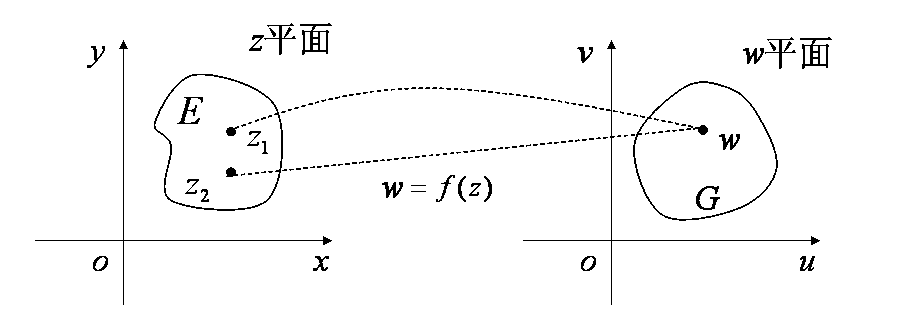
\includegraphics[keepaspectratio,alt={图2.1 复变函数的映射}]{figures/02-解析函数/fig-p03-a37f4956.png}}
\caption{图2.1 复变函数的映射}
\end{figure}

\subsubsection{反函数}\label{ux53cdux51fdux6570}

设函数 \(w=f(z)\) 定义在 \(E\) 上，值域为 \(G\)。若对于 \(G\) 中的任一点
\(w\)，在 \(E\) 中存在一个或几个点 \(z\) 与之对应，则在 \(G\)
上确定了一个单值或多值函数，记作 \(z=f^{-1}(w)\)，称为函数 \(w=f(z)\)
的\textbf{反函数}。

\textbf{例 2.1} 函数 \(\displaystyle w=\frac{1}{z}\) 将 \(z\)
平面上的直线 \(x=1\) 变成 \(w\) 平面上的何种曲线？

\textbf{解} 令 \(z=x+iy\)，\(w=u+iv\)，则

\[
w=u+iv=\frac{1}{z}=\frac{1}{x+iy}=\frac{x-iy}{x^2+y^2},
\]

故

\[
u=\frac{x}{x^2+y^2},\qquad v=-\frac{y}{x^2+y^2}.
\]

\(z\) 平面上的直线 \(x=1\) 对应于 \(w\) 平面上的曲线

\[
u=\frac{1}{1+y^2},\qquad v=-\frac{y}{1+y^2}.
\]

于是

\[
u^2+v^2
=\frac{1}{(1+y^2)^2}+\frac{y^2}{(1+y^2)^2}
=\frac{1}{1+y^2}=u,
\]

即

\[
\left(u-\frac{1}{2}\right)^2+v^2=\frac{1}{4}.
\]

所以直线 \(x=1\) 被映射为 \(w\) 平面上以 \(\left(\dfrac{1}{2},0\right)\)
为圆心、\(\dfrac{1}{2}\) 为半径的圆。

\begin{figure}
\centering
\pandocbounded{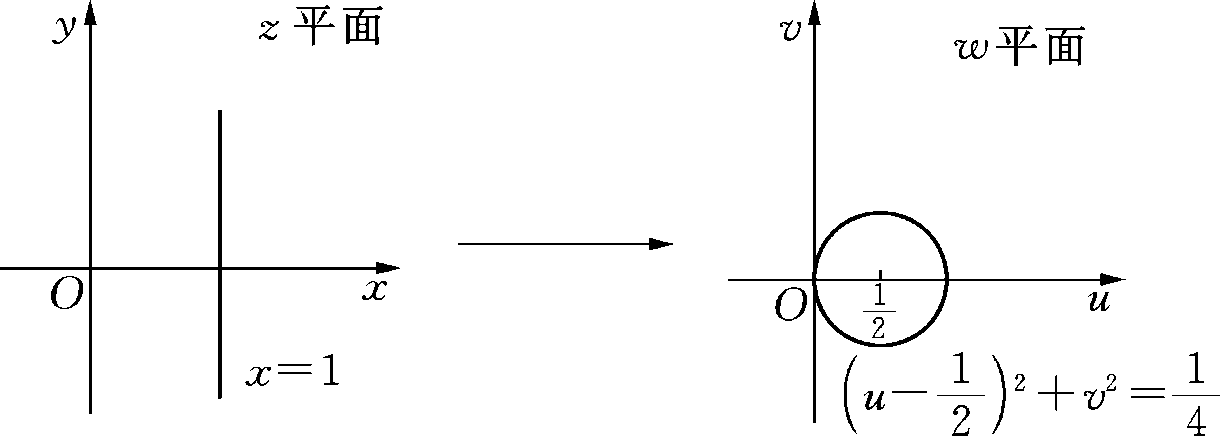
\includegraphics[keepaspectratio,alt={图2.2 例2.1 直线 x=1 的像}]{figures/02-解析函数/fig-p04-7f4c02e9.png}}
\caption{图2.2 例2.1 直线 x=1 的像}
\end{figure}

\subsection{2.1.2
复变函数的极限}\label{ux590dux53d8ux51fdux6570ux7684ux6781ux9650}

\textbf{定义 2.2} 设函数 \(w=f(z)\) 定义在 \(z_0\) 的去心邻域
\(0<|z-z_0|<r\) 内。若存在常数 \(A\)，对于任意给定的
\(\varepsilon>0\)，都存在一正数 \(\delta\)（\(0<\delta\le r\)），使得当
\(0<|z-z_0|<\delta\) 时，有

\[
|f(z)-A|<\varepsilon,
\]

则称函数 \(f(z)\) 当 \(z\to z_0\) 时的极限存在，常数 \(A\)
为其极限值，记作

\[
\lim_{z\to z_0}f(z)=A
\qquad\text{或}\qquad
f(z)\to A\ (z\to z_0).
\]

\textbf{几何意义} 当变点 \(z\) 进入 \(z_0\)
的充分小的去心邻域时，它的像点 \(f(z)\) 就落入 \(A\)
的一个预先给定的邻域内。

\begin{quote}
定义中 \(z\to z_0\) 的方式是任意的：\(z\) 在 \(z_0\)
的去心邻域内沿任何曲线以任何方式趋于 \(z_0\) 时，\(f(z)\)
都要趋向于同一个常数 \(A\)。
\end{quote}

\begin{figure}
\centering
\pandocbounded{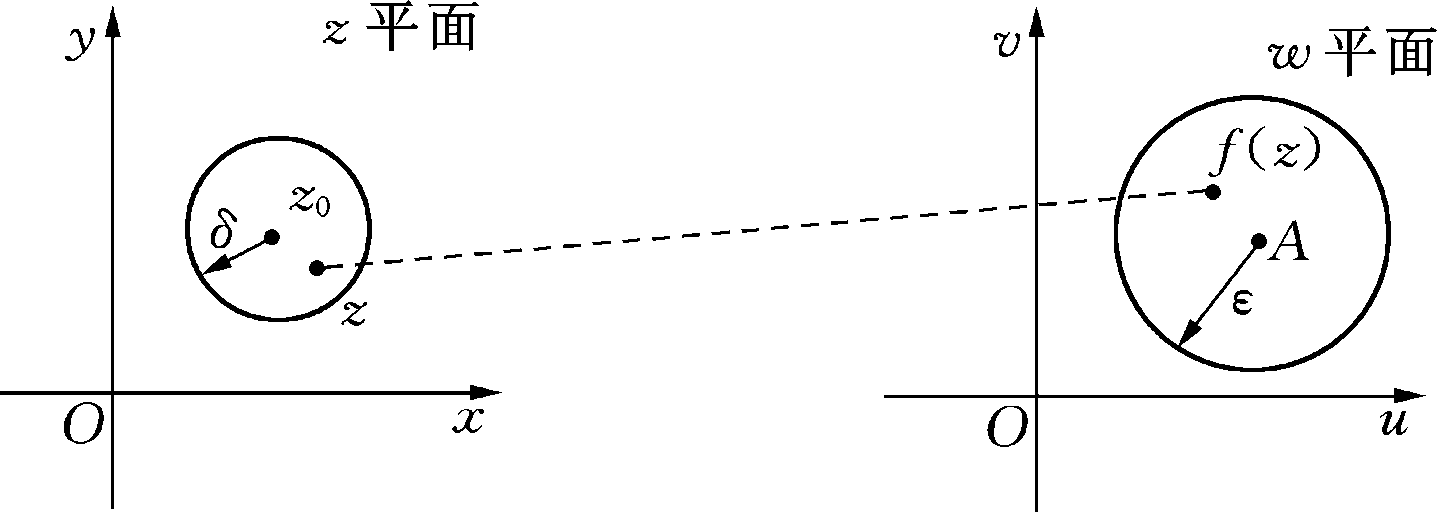
\includegraphics[keepaspectratio,alt={图2.3 极限的几何意义}]{figures/02-解析函数/fig-p06-bc429569.png}}
\caption{图2.3 极限的几何意义}
\end{figure}

\textbf{定理 2.1} 设
\(f(z)=u(x,y)+iv(x,y)\)，\(z_0=x_0+iy_0\)，\(A=a+ib\)，则

\[
\lim_{z\to z_0}f(z)=A
\iff
\lim_{(x,y)\to(x_0,y_0)}u(x,y)=a,\quad
\lim_{(x,y)\to(x_0,y_0)}v(x,y)=b .
\]

\textbf{证明要点}

\begin{itemize}
\tightlist
\item
  \textbf{必要性}：设 \(\lim_{z\to z_0}f(z)=A\)，即对任意
  \(\varepsilon>0\)，存在 \(\delta>0\)，当
\end{itemize}

\[
0<|z-z_0|=\sqrt{(x-x_0)^2+(y-y_0)^2}<\delta
\]

时，有

\[
|f(z)-A|=\sqrt{(u-a)^2+(v-b)^2}<\varepsilon .
\]

由于
\(|u-a|\le\sqrt{(u-a)^2+(v-b)^2}\)，\(|v-b|\le\sqrt{(u-a)^2+(v-b)^2}\)，故
\(|u-a|<\varepsilon\)、\(|v-b|<\varepsilon\)，从而两个实函数极限成立。

\begin{itemize}
\tightlist
\item
  \textbf{充分性}：设两个实函数极限成立，则当
  \(\sqrt{(x-x_0)^2+(y-y_0)^2}<\delta\) 时，有
  \(|u-a|<\frac{\varepsilon}{2}\)，\(|v-b|<\frac{\varepsilon}{2}\)，所以
\end{itemize}

\[
|f(z)-A|=|(u-a)+i(v-b)|\le|u-a|+|v-b|<\varepsilon ,
\]

即 \(\lim_{z\to z_0}f(z)=A\)。

\textbf{定理 2.2（极限运算法则）} 若

\[
\lim_{z\to z_0}f(z)=A,\qquad \lim_{z\to z_0}g(z)=B,
\]

则

\[
(1)\ \lim_{z\to z_0}\bigl(f(z)\pm g(z)\bigr)=A\pm B;\qquad
(2)\ \lim_{z\to z_0}f(z)\cdot g(z)=AB;
\]

\[
(3)\ \lim_{z\to z_0}\frac{f(z)}{g(z)}=\frac{A}{B}\quad (B\neq 0).
\]

\textbf{例 2.2}
判断下列函数在原点处的极限是否存在，若存在，试求出极限值：

\[
(1)\ f(z)=\frac{z\operatorname{Re}(z)}{|z|};\qquad
(2)\ f(z)=\frac{\operatorname{Re}(z^2)}{|z|^2}.
\]

\textbf{解}

\textbf{(1) 方法一} 因为

\[
|f(z)|=\left|z\frac{\operatorname{Re}(z)}{z}\right|\le |z|,
\]

所以对任意 \(\varepsilon>0\)，取 \(\delta=\varepsilon\)，当
\(0<|z|<\delta\) 时，总有

\[
|f(z)-0|=|f(z)|\le|z|<\varepsilon .
\]

根据极限定义，\(\lim_{z\to0}f(z)=0\)。

\textbf{(1) 方法二} 设 \(z=x+iy\)，则

\[
f(z)=\frac{(x+iy)x}{\sqrt{x^2+y^2}}
=\frac{x^2}{\sqrt{x^2+y^2}}+i\frac{xy}{\sqrt{x^2+y^2}},
\]

故

\[
u(x,y)=\frac{x^2}{\sqrt{x^2+y^2}},\qquad
v(x,y)=\frac{xy}{\sqrt{x^2+y^2}},
\]

且

\[
\lim_{(x,y)\to(0,0)}u=0,\qquad \lim_{(x,y)\to(0,0)}v=0 .
\]

由定理 2.1，得 \(\lim_{z\to0}f(z)=0\)。

\textbf{(2) 方法一} 设 \(z=x+iy\)，则

\[
z^2=x^2-y^2+2xyi,\qquad |z|^2=x^2+y^2,
\]

故

\[
f(z)=\frac{\operatorname{Re}(z^2)}{|z|^2}=\frac{x^2-y^2}{x^2+y^2},\qquad
u(x,y)=\frac{x^2-y^2}{x^2+y^2},\quad v(x,y)=0 .
\]

让 \(z\) 沿直线 \(y=kx\) 趋向于 \(0\)，有

\[
\lim_{(x,y)\to(0,0)}u(x,y)=\lim_{x\to0}\frac{x^2-k^2x^2}{x^2+k^2x^2}
=\frac{1-k^2}{1+k^2}.
\]

极限随 \(k\) 变化而不同，所以 \(\lim_{z\to0}f(z)\) 不存在。

\textbf{(2) 方法二} 设 \(z=re^{i\theta}\)，则

\[
f(z)=\frac{r^2\cos 2\theta}{r^2}=\cos 2\theta .
\]

让 \(z\) 沿不同射线 \(\arg z=\theta\) 趋向于 \(0\) 时，\(f(z)\)
趋向于不同的值，所以极限不存在。

\subsection{2.1.3
复变函数的连续性}\label{ux590dux53d8ux51fdux6570ux7684ux8fdeux7eedux6027}

\textbf{定义 2.3} 若

\[
\lim_{z\to z_0}f(z)=f(z_0),
\]

则说函数 \(f(z)\) 在点 \(z_0\) 处连续。如果函数 \(f(z)\) 在区域 \(D\)
内每一点都连续，那么称函数 \(f(z)\) 在区域 \(D\) 内连续。

\textbf{定理 2.3} 若 \(f(z)\)、\(g(z)\) 在点 \(z_0\)
连续，则其和、差、积、商（要求分母不为零）在点 \(z_0\) 处连续。特别地：

\begin{itemize}
\tightlist
\item
  \begin{enumerate}
  \def\labelenumi{(\arabic{enumi})}
  \tightlist
  \item
    多项式 \(\displaystyle w=a_0z^n+a_1z^{n-1}+\cdots+a_{n-1}z+a_n\)
    在整个复平面上连续；
  \end{enumerate}
\item
  \begin{enumerate}
  \def\labelenumi{(\arabic{enumi})}
  \setcounter{enumi}{1}
  \tightlist
  \item
    任何一个有理分式函数
    \(\displaystyle w=\frac{a_0z^n+a_1z^{n-1}+\cdots+a_{n-1}z+a_n}{b_0z^m+b_1z^{m-1}+\cdots+b_{m-1}z+b_m}\)
    在复平面上除去使分母为零的点外处处连续。
  \end{enumerate}
\end{itemize}

\textbf{定理 2.4} 若函数 \(h=g(z)\) 在点 \(z_0\) 连续，函数
\(\varphi=f(h)\) 在 \(h_0=g(z_0)\) 连续，则复合函数 \(\varphi=f(g(z))\)
在 \(z_0\) 处连续。

\textbf{定理 2.5} 设函数

\[
f(z)=u(x,y)+iv(x,y),\qquad z_0=x_0+iy_0,
\]

则 \(f(z)\) 在点 \(z_0\) 连续的充分必要条件是 \(u(x,y)\)、\(v(x,y)\)
均在点 \((x_0,y_0)\) 处连续。

\textbf{例 2.3} 讨论函数 \(\arg z\) 的连续性。

\textbf{解}

\begin{itemize}
\tightlist
\item
  当 \(z=0\) 时，\(\arg z\) 无定义，因而不连续。
\item
  当 \(z_0\) 为负实轴上的点，即 \(z_0=x_0<0\) 时：
\end{itemize}

\[
\lim_{y\to0^-,\,z\to z_0}\arg z=\lim_{y\to0^-,\,x\to x_0}\left(\arctan\frac{y}{x}-\pi\right)=-\pi,
\]

\[
\lim_{y\to0^+,\,z\to z_0}\arg z=\lim_{y\to0^+,\,x\to x_0}\left(\arctan\frac{y}{x}+\pi\right)=\pi,
\]

左右极限不等，故 \(\arg z\) 在负实轴上不连续。

\begin{itemize}
\tightlist
\item
  若 \(z_0=x_0+iy_0\) 不是原点也不是负实轴及虚轴上的点，设
  \(x_0\neq 0\)，则
\end{itemize}

\[
\arg z=
\begin{cases}
\arctan(y/x),\\
\arctan(y/x)\pm\pi,
\end{cases}
\]

且

\[
\lim_{z\to z_0}\arg z
=\lim_{(x,y)\to(x_0,y_0)}
\begin{cases}
\arctan(y/x),\\
\arctan(y/x)\pm\pi
\end{cases}
=
\begin{cases}
\arctan(y_0/x_0),\\
\arctan(y_0/x_0)\pm\pi
\end{cases}
=\arg z_0 .
\]

故 \(\lim_{z\to z_0}\arg z=\arg z_0\)，即 \(\arg z\)
在除去原点和负实轴及虚轴的复平面上连续。

\begin{itemize}
\tightlist
\item
  当 \(z_0\) 为正、负虚轴上的点 \(z_0=iy_0\)（\(y_0\neq 0\)）时，
\end{itemize}

\[
\lim_{z\to z_0}\arg z=\pm\frac{\pi}{2}=\arg z_0,
\]

故 \(\arg z\) 在虚轴上也连续。

因此 \(\arg z\) 在复平面上除了原点和负实轴外连续。

\textbf{补充（连续函数的有界性）} 设 \(\overline D\)
为复平面上的有界闭区域，函数 \(w=f(z)\) 在 \(\overline D\)
上连续，则函数 \(f(z)\) 在 \(\overline D\) 上有界，即存在常数
\(M\)，使对于 \(\forall z\in\overline D\)，都有
\(|f(z)|\le M\)。在闭曲线或包含曲线端点在内的曲线段上连续的函数 \(f(z)\)
在曲线上有界，即 \(|f(z)|\le M\)。

\subsection{常见错误与注意点}\label{ux5e38ux89c1ux9519ux8befux4e0eux6ce8ux610fux70b9-3}

\begin{enumerate}
\def\labelenumi{\arabic{enumi}.}
\tightlist
\item
  \textbf{极限定义中 \(z\to z_0\) 具有任意性}：\(z\) 沿任何路径趋于
  \(z_0\) 都必须趋向同一常数
  \(A\)。仅沿个别路径（如直线）极限存在不能说明极限存在；反之，沿两条路径得到不同值则极限一定不存在。
\item
  \textbf{\(\operatorname{Re}(z)\)、\(\operatorname{Im}(z)\)、\(\bar z\)、\(|z|\)
  常常不是``好''函数}：判断其极限、可导性时，常需借助实部/虚部或两条路径验证。
\item
  \textbf{\(\arg z\) 的连续性}：\(\arg z\)
  在原点无定义，在负实轴处左右极限不等，故负实轴是间断线；实轴、虚轴其余点连续。
\item
  \textbf{复变函数的极限}：先化为 \(u(x,y)\)、\(v(x,y)\)
  两个二元实函数极限，再借助定理 2.1 判断，往往更简便。
\end{enumerate}

\subsection{本节小结}\label{ux672cux8282ux5c0fux7ed3-3}

\begin{itemize}
\tightlist
\item
  复变函数 \(w=f(z)=u(x,y)+iv(x,y)\)：定义域 \(E\)、值域
  \(f(E)=G\)、映射、像与原像、单值/多值、反函数。
\item
  复变函数的极限：\(\varepsilon\)-\(\delta\)
  定义；\(\lim_{z\to z_0}f(z)=A \iff\) 实部、虚部同时收敛。
\item
  极限运算法则：和差积商。
\item
  连续性：逐点连续、区域连续；和差积商连续；复合连续；\(u,v\) 同时连续
  \(\iff f\) 连续。
\item
  典型结论：\(\arg z\)
  在除去原点和负实轴外连续；连续函数在有界闭区域上有界。
\end{itemize}

\section{§2.2
解析函数的概念}\label{ux89e3ux6790ux51fdux6570ux7684ux6982ux5ff5}

\begin{quote}
\textbf{本节目标}：掌握复变函数导数的定义，会用定义求简单函数的导数；理解``可导''与``解析''的联系与区别；掌握常用求导法则；会用定义判断函数的可导性与解析性，会求函数的奇点。
\textbf{本节重点}：导数的极限定义；求导法则；解析函数与奇点的概念。
\textbf{本节难点}：可导与解析的区别；用两条路径判断可导性；\(f(z)=z\operatorname{Re}(z)\)、\(\bar z\)
等的可导性。
\end{quote}

\subsection{2.2.1
复变函数的导数}\label{ux590dux53d8ux51fdux6570ux7684ux5bfcux6570}

\textbf{定义 2.4（导数的定义）} 设函数 \(w=f(z)\) 定义在 \(z\)
平面上区域 \(D\) 内，点
\(z_0\)、\(z_0+\Delta z\in D\)，\(\Delta w=f(z_0+\Delta z)-f(z_0)\)，若极限

\[
\lim_{\Delta z\to0}\frac{\Delta w}{\Delta z}
=\lim_{\Delta z\to0}\frac{f(z_0+\Delta z)-f(z_0)}{\Delta z}
\]

存在，则称函数 \(f(z)\) 在 \(z_0\) 可导，这个极限值称为 \(f(z)\) 在
\(z_0\) 的导数，记作

\[
f'(z_0)=\left.\frac{\mathrm{d}f(z)}{\mathrm{d}z}\right|_{z=z_0}
=\left.\frac{\mathrm{d}w}{\mathrm{d}z}\right|_{z=z_0}
=\lim_{\Delta z\to0}\frac{f(z_0+\Delta z)-f(z_0)}{\Delta z}.
\]

若函数 \(f(z)\) 在区域 \(D\) 内每一点都可导，则称函数 \(f(z)\) 在区域
\(D\) 内可导。

\begin{quote}
\textbf{注意}：复变函数的自变量与增量都是复数，\(\Delta z\to0\)
的方式是任意的（可在复平面内沿任意曲线趋于 \(0\)）。
\end{quote}

\textbf{例 2.4} 求函数 \(f(z)=z^n\)（\(n\) 为正整数）的导数。

\textbf{解}

\[
\begin{aligned}
\frac{\mathrm{d}f(z)}{\mathrm{d}z}
&=\lim_{\Delta z\to0}\frac{(z+\Delta z)^n-z^n}{\Delta z}\\
&=\lim_{\Delta z\to0}\left(C_n^1z^{n-1}+C_n^2z^{n-2}\Delta z+\cdots+C_n^{n-1}z\Delta z^{n-2}+C_n^n\Delta z^{n-1}\right)\\
&=C_n^1z^{n-1}=nz^{n-1}.
\end{aligned}
\]

故

\[
f'(z)=nz^{n-1}.
\]

这说明 \(z^n\)（\(n\) 为正整数）在整个 \(z\) 平面上处处可导。

\textbf{例 2.5} 考察函数 \(f(z)=\dfrac{1}{z}\) 在整个 \(z\)
平面上的可导性。

\textbf{解} 当 \(z\neq 0\) 时，

\[
\begin{aligned}
\lim_{\Delta z\to0}\frac{f(z+\Delta z)-f(z)}{\Delta z}
&=\lim_{\Delta z\to0}\frac{\dfrac{1}{z+\Delta z}-\dfrac{1}{z}}{\Delta z}
=\lim_{\Delta z\to0}\frac{-1}{z^2+z\Delta z}\\
&=-\frac{1}{z^2},
\end{aligned}
\]

即

\[
f'(z)=-\frac{1}{z^2}\quad (z\neq 0).
\]

所以函数在整个 \(z\) 平面上除去原点外处处可导。

\textbf{例 2.6} 研究函数 \(f(z)=\bar z\) 在整个 \(z\) 平面上的可导性。

\textbf{解} 令 \(z=x+iy\)，\(\Delta z=\Delta x+i\Delta y\)，则

\[
\lim_{\Delta z\to0}\frac{f(z+\Delta z)-f(z)}{\Delta z}
=\lim_{\Delta z\to0}\frac{\overline{z+\Delta z}-\bar z}{\Delta z}
=\lim_{\Delta z\to0}\frac{\overline{\Delta z}}{\Delta z}
=\lim_{\Delta z\to0}\frac{\Delta x-i\Delta y}{\Delta x+i\Delta y}.
\]

让 \(z+\Delta z\) 沿着平行于 \(x\) 轴的直线趋于 \(z\)，此时
\(\Delta y=0\)：

\[
\lim_{\Delta z\to0}\frac{\Delta x-i\Delta y}{\Delta x+i\Delta y}
=\lim_{\Delta x\to0}\frac{\Delta x}{\Delta x}=1 .
\]

让 \(z+\Delta z\) 沿着平行于 \(y\) 轴的直线趋于 \(z\)，此时
\(\Delta x=0\)：

\[
\lim_{\Delta z\to0}\frac{\Delta x-i\Delta y}{\Delta x+i\Delta y}
=\lim_{\Delta y\to0}\frac{-i\Delta y}{i\Delta y}=-1 .
\]

两条路径极限不同，故函数在整个 \(z\) 平面上处处不可导。

\subsubsection{可导必连续}\label{ux53efux5bfcux5fc5ux8fdeux7eed}

若函数 \(f(z)\) 在点 \(z_0\) 可导，按导数定义，用极限语言表达：对任意
\(\varepsilon>0\)，必定存在 \(\delta>0\)，使得当 \(0<|\Delta z|<\delta\)
时，有

\[
\left|\frac{f(z_0+\Delta z)-f(z_0)}{\Delta z}-f'(z_0)\right|<\varepsilon .
\]

令

\[
\alpha(\Delta z)=\frac{f(z_0+\Delta z)-f(z_0)}{\Delta z}-f'(z_0),
\]

则 \(|\alpha(\Delta z)|<\varepsilon\)，于是
\(\lim_{\Delta z\to0}\alpha(\Delta z)=0\)。又因为

\[
f(z_0+\Delta z)-f(z_0)=f'(z_0)\Delta z+\alpha(\Delta z)\Delta z,
\]

所以

\[
\lim_{\Delta z\to0}\left(f(z_0+\Delta z)-f(z_0)\right)=0,
\]

即 \(f(z)\) 在 \(z_0\) 连续。\textbf{（可导必然连续，但连续未必可导。）}

\subsubsection{常用的求导公式与法则}\label{ux5e38ux7528ux7684ux6c42ux5bfcux516cux5f0fux4e0eux6cd5ux5219}

设 \(C\) 为复常数，\(n\) 为正整数，\(f(z)\)、\(g(z)\) 可导：

\[
(1)\ (C)'=0;
\]

\[
(2)\ (z^n)'=nz^{n-1};
\]

\[
(3)\ \bigl(f(z)\pm g(z)\bigr)'=f'(z)\pm g'(z);
\]

\[
(4)\ \bigl(f(z)g(z)\bigr)'=f'(z)g(z)+f(z)g'(z);
\]

\[
(5)\ \left(\frac{f(z)}{g(z)}\right)'=\frac{f'(z)g(z)-f(z)g'(z)}{g^2(z)}\quad (g(z)\neq 0);
\]

\[
(6)\ \bigl(f(g(z))\bigr)'=f'(w)g'(z),\qquad w=g(z);
\]

\[
(7)\ \text{若 }w=f(z)\text{ 与 }z=h(w)\text{ 互为反函数，且 }h'(w)\neq 0,\text{ 则 }f'(z)=\frac{1}{h'(w)}.
\]

\begin{quote}
\textbf{公式疑难提醒}：课件中商法则一处写作分子为
\(f'(z)g(z)+f(z)g'(z)\)（即乘积法则形式）。这里按数学上正确的商法则写成
\(f'(z)g(z)-f(z)g'(z)\)，请以减号为准。
\end{quote}

\subsection{2.2.2
解析函数的概念}\label{ux89e3ux6790ux51fdux6570ux7684ux6982ux5ff5-1}

\textbf{定义 2.5} 若函数 \(f(z)\) 在点 \(z_0\) 及 \(z_0\)
的邻域内处处可导，则称函数 \(f(z)\) 在点 \(z_0\) \textbf{解析}。若函数
\(f(z)\) 在区域 \(D\) 内每一点都解析，则称函数 \(f(z)\) 在区域 \(D\)
内解析，或称 \(f(z)\) 是 \(D\) 内的解析函数。

若 \(f(z)\) 在点 \(z_0\) 不解析，但在 \(z_0\) 的任一邻域内总有 \(f(z)\)
的解析点，则称 \(z_0\) 为 \(f(z)\) 的\textbf{奇点}。

\textbf{例 2.7} 研究函数 \(f(z)=z\operatorname{Re}(z)\) 的解析性。

\textbf{解} 设 \(z=x+iy\)，\(z_0=x_0+iy_0\)。当 \(z_0\neq 0\) 时，

\[
\lim_{z\to z_0}\frac{\Delta w}{\Delta z}
=\lim_{z\to z_0}\frac{z\operatorname{Re}(z)-z_0\operatorname{Re}(z_0)}{z-z_0}.
\]

添项化简：

\[
\begin{aligned}
&\lim_{z\to z_0}\frac{z\operatorname{Re}(z)-z_0\operatorname{Re}(z_0)}{z-z_0}\\
&=\lim_{z\to z_0}\left(\frac{z\operatorname{Re}(z)-z_0\operatorname{Re}(z)}{z-z_0}
+\frac{z_0\operatorname{Re}(z)-z_0\operatorname{Re}(z_0)}{z-z_0}\right)\\
&=\lim_{z\to z_0}\left(x+z_0\frac{x-x_0}{z-z_0}\right).
\end{aligned}
\]

令 \(x=x_0\), \(y\to y_0\)，则

\[
\lim_{(x,y)\to(x_0,y_0)}\frac{\Delta w}{\Delta z}=x_0 .
\]

令 \(y=y_0\), \(x\to x_0\)，则

\[
\lim_{(x,y)\to(x_0,y_0)}\frac{\Delta w}{\Delta z}=x_0+iy_0 .
\]

两者不同（当 \(z_0\neq0\) 时），故 \(f(z)=z\operatorname{Re}(z)\) 当
\(z\neq0\) 时不可导。

当 \(z_0=0\) 时，

\[
\lim_{z\to0}\frac{\Delta w}{\Delta z}
=\lim_{z\to0}\frac{z\operatorname{Re}(z)}{z}
=\lim_{z\to0}\operatorname{Re}(z)=0 .
\]

故函数仅在 \(z=0\) 处导数存在，它在 \(z\) 平面上处处不解析。

\textbf{例 2.8} 研究分式线性函数

\[
w=\frac{az+b}{cz+d}
\]

的解析性，式中 \(a,b,c,d\) 为复常数，且 \(ad-bc\neq 0\)。

\textbf{解} 由导数的运算法则，除了使得分母为零的点 \(z=-d/c\)
外，这个函数在复平面上处处可导。因此，除了点 \(z=-d/c\)
外，它在复平面上处处解析，且

\[
w'=\frac{a(cz+d)-c(az+b)}{(cz+d)^2}=\frac{ad-bc}{(cz+d)^2}.
\]

\textbf{定理 2.6}

\begin{itemize}
\tightlist
\item
  \begin{enumerate}
  \def\labelenumi{(\arabic{enumi})}
  \tightlist
  \item
    在区域 \(D\) 内解析的两个函数 \(f(z)\) 和
    \(g(z)\)，其和、差、积、商（要求分母不为零）在区域 \(D\) 内解析。
  \end{enumerate}
\item
  \begin{enumerate}
  \def\labelenumi{(\arabic{enumi})}
  \setcounter{enumi}{1}
  \tightlist
  \item
    设函数 \(h=g(z)\) 在 \(z\) 平面上的区域 \(D\) 内解析，函数
    \(\varphi=f(h)\) 在 \(h\) 平面上的区域 \(D^*\) 内解析。若对于 \(D\)
    内每一点 \(z\)，\(g(z)\) 的对应值 \(h\) 落在 \(D^*\) 内，则复合函数
    \(\varphi=f(g(z))\) 在区域 \(D\) 内解析。
  \end{enumerate}
\end{itemize}

\subsection{常见错误与注意点}\label{ux5e38ux89c1ux9519ux8befux4e0eux6ce8ux610fux70b9-4}

\begin{enumerate}
\def\labelenumi{\arabic{enumi}.}
\tightlist
\item
  \textbf{可导与解析不同}：在一点可导不一定在该点解析（解析要求在该点及其邻域内处处可导）；在区域
  \(D\) 内可导等价于在 \(D\) 内解析。
\item
  \textbf{\(\Delta z\to0\) 的任意性}：复变函数求导时 \(\Delta z\)
  必须能以任意方式趋于 \(0\)，因此仅沿实轴或虚轴验证不够。
\item
  \textbf{商法则}：注意分子应为
  \(f'(z)g(z)-f(z)g'(z)\)，不要与乘积法则混淆。
\item
  \textbf{奇点}：如 \(f(z)=z\operatorname{Re}(z)\) 仅在 \(z=0\)
  可导，\(z=0\) 是奇点（其余点不可导也不解析）。
\end{enumerate}

\subsection{本节小结}\label{ux672cux8282ux5c0fux7ed3-4}

\begin{itemize}
\tightlist
\item
  导数：\(\displaystyle f'(z_0)=\lim_{\Delta z\to0}\frac{f(z_0+\Delta z)-f(z_0)}{\Delta z}\)；可导
  \(\Rightarrow\) 连续。
\item
  常用求导公式：\(\left(z^n\right)'=nz^{n-1}\)、\(\left(\frac{1}{z}\right)'=-\frac{1}{z^2}\)、和差积商、复合、反函数。
\item
  解析：在点及邻域处处可导；在区域 \(D\)
  内处处解析；解析函数和差积商（分母非零）仍解析；复合解析。
\item
  典型反例：\(\bar z\) 处处不可导；\(z\operatorname{Re}(z)\) 仅在
  \(z=0\) 可导、处处不解析；\(\frac{az+b}{cz+d}\) 除 \(z=-d/c\) 外解析。
\end{itemize}

\section{§2.3
函数可导与解析的充要条件}\label{ux51fdux6570ux53efux5bfcux4e0eux89e3ux6790ux7684ux5145ux8981ux6761ux4ef6}

\begin{quote}
\textbf{本节目标}：掌握柯西-黎曼（C-R）方程；理解复变函数可导（解析）的充要条件；能利用
C-R 方程判断函数的可导性、解析性，并求出导数。 \textbf{本节重点}：C-R
方程及其使用；定理 2.7 的证明思路；函数导数公式的四种形式。
\textbf{本节难点}：可导的充要条件中``可微 + C-R
方程''的直观理解；证明中高阶无穷小量、复合函数极限的处理。
\end{quote}

\subsection{2.3.1
柯西-黎曼方程}\label{ux67efux897f-ux9eceux66fcux65b9ux7a0b}

\textbf{定义 2.6} 对于二元实函数 \(u(x,y)\) 和 \(v(x,y)\)，方程

\[
\frac{\partial u}{\partial x}=\frac{\partial v}{\partial y},\qquad
\frac{\partial u}{\partial y}=-\frac{\partial v}{\partial x}
\]

称为\textbf{柯西-黎曼方程}（简记为 \textbf{C-R 方程}）。

\subsection{2.3.2
可导的充要条件}\label{ux53efux5bfcux7684ux5145ux8981ux6761ux4ef6}

\textbf{定理 2.7} 设函数 \(f(z)=u(x,y)+iv(x,y)\) 在区域 \(D\)
内有定义，则 \(f(z)\) 在区域 \(D\) 内一点 \(z=x+iy\) 可导的充要条件是：

\[
(1)\ u(x,y),v(x,y)\text{ 在点 }(x,y)\text{ 可微};\qquad
(2)\ u(x,y),v(x,y)\text{ 在点 }(x,y)\text{ 满足 C-R 方程}.
\]

\textbf{证明}

\textbf{先证必要性。} 设 \(f(z)\) 在区域 \(D\) 内一点 \(z=x+iy\)
可导，由可导的定义有

\[
\Delta w=f'(z)\Delta z+\alpha(\Delta z)\Delta z,\qquad \alpha(\Delta z)\to0\ (\Delta z\to0).
\]

令

\[
\Delta w=\Delta u+i\Delta v,\qquad \Delta z=\Delta x+i\Delta y,\qquad f'(z)=\alpha+i\beta,
\]

则

\[
\Delta u+i\Delta v=(\alpha+i\beta)(\Delta x+i\Delta y)+\alpha(\Delta z)\Delta z .
\]

再令

\[
\varepsilon_1=\operatorname{Re}\bigl(\alpha(\Delta z)\Delta z\bigr),\qquad
\varepsilon_2=\operatorname{Im}\bigl(\alpha(\Delta z)\Delta z\bigr),
\]

则 \(\varepsilon_1,\varepsilon_2\) 都是关于
\(\sqrt{\Delta x^2+\Delta y^2}\) 的高阶无穷小量，并且

\[
\Delta u=\alpha\Delta x-\beta\Delta y+\varepsilon_1,\qquad
\Delta v=\beta\Delta x+\alpha\Delta y+\varepsilon_2 .
\]

根据二元实函数微分的定义，\(u(x,y)\) 与 \(v(x,y)\) 在点 \((x,y)\)
可微，并且有

\[
\alpha=\frac{\partial u}{\partial x}=\frac{\partial v}{\partial y},\qquad
\beta=-\frac{\partial u}{\partial y}=\frac{\partial v}{\partial x},
\]

这正是 C-R 方程。

\textbf{再证充分性。} 已知 \(u(x,y)\) 和 \(v(x,y)\) 在点 \((x,y)\)
可微，即有

\[
\Delta u=\frac{\partial u}{\partial x}\Delta x+\frac{\partial u}{\partial y}\Delta y+\varepsilon_1,\qquad
\Delta v=\frac{\partial v}{\partial x}\Delta x+\frac{\partial v}{\partial y}\Delta y+\varepsilon_2,
\]

其中 \(\varepsilon_1,\varepsilon_2\) 都是关于
\(\sqrt{\Delta x^2+\Delta y^2}\) 的高阶无穷小量，于是

\[
\begin{aligned}
\Delta w
&=\bigl(u(x+\Delta x,y+\Delta y)-u(x,y)\bigr)+i\bigl(v(x+\Delta x,y+\Delta y)-v(x,y)\bigr)\\
&=\Delta u+i\Delta v,
\end{aligned}
\]

所以

\[
\frac{\Delta w}{\Delta z}
=\frac{\Delta u+i\Delta v}{\Delta x+i\Delta y}
=\frac{\left(\dfrac{\partial u}{\partial x}\Delta x+\dfrac{\partial u}{\partial y}\Delta y\right)+
i\left(\dfrac{\partial v}{\partial x}\Delta x+\dfrac{\partial v}{\partial y}\Delta y\right)}
{\Delta x+i\Delta y}+\varepsilon,
\]

其中

\[
\varepsilon=\frac{\varepsilon_1+i\varepsilon_2}{\Delta x+i\Delta y},\qquad
|\varepsilon|\le\frac{|\varepsilon_1|+|\varepsilon_2|}{\sqrt{\Delta x^2+\Delta y^2}}\to0 .
\]

由于 \(u,v\) 满足 C-R 方程，分子可整理为

\[
\left(\frac{\partial u}{\partial x}+i\frac{\partial v}{\partial x}\right)(\Delta x+i\Delta y),
\]

故

\[
\lim_{\Delta z\to0}\frac{\Delta w}{\Delta z}
=\frac{\partial u}{\partial x}+i\frac{\partial v}{\partial x}.
\]

即 \(f(z)=u+iv\) 在点 \(z=x+iy\) 可导。\(\qquad\square\)

\subsubsection{函数导数公式的四种形式}\label{ux51fdux6570ux5bfcux6570ux516cux5f0fux7684ux56dbux79cdux5f62ux5f0f}

\[
f'(z)=\frac{\partial u}{\partial x}+i\frac{\partial v}{\partial x}
=\frac{\partial v}{\partial y}-i\frac{\partial u}{\partial y}
=\frac{\partial u}{\partial x}-i\frac{\partial u}{\partial y}
=\frac{\partial v}{\partial y}+i\frac{\partial v}{\partial x}.
\]

\subsection{2.3.3
解析的充要条件}\label{ux89e3ux6790ux7684ux5145ux8981ux6761ux4ef6}

\textbf{定理 2.8} 函数 \(f(z)=u(x,y)+iv(x,y)\) 在区域 \(D\)
内解析的充要条件是：

\[
(1)\ u(x,y),v(x,y)\text{ 在 }D\text{ 内可微};\qquad
(2)\ u(x,y),v(x,y)\text{ 在 }D\text{ 内满足 C-R 方程}.
\]

\textbf{推论 2.1} 若 \(u(x,y)\) 与 \(v(x,y)\) 的一阶偏导在点
\((x,y)\)（或区域 \(D\) 内）存在而且连续，并满足 C-R 方程，则 \(f(z)\)
在点 \((x,y)\) 可导（或在区域 \(D\) 内解析）。

\subsection{2.3.4 例题}\label{ux4f8bux9898}

\textbf{例 2.9} 讨论下列函数的可导性与解析性：

\[
(1)\ f(z)=\operatorname{Im}(z);\qquad (2)\ f(z)=|z|^2z .
\]

\textbf{解}

\textbf{(1)} 设 \(z=x+iy\)，则 \(f(z)=\operatorname{Im}(z)=y\)，故

\[
u(x,y)=y,\qquad v(x,y)=0,
\]

且

\[
\frac{\partial u}{\partial x}=0,\quad
\frac{\partial u}{\partial y}=1,\quad
\frac{\partial v}{\partial x}=0,\quad
\frac{\partial v}{\partial y}=0 .
\]

\(u,v\) 在复平面上可微，但不满足 C-R 方程，所以
\(f(z)=\operatorname{Im}(z)\) 在复平面上处处不可导、处处不解析。

\textbf{(2)} 设 \(z=x+iy\)，则

\[
f(z)=(x^2+y^2)x+i(x^2+y^2)y .
\]

故

\[
u(x,y)=(x^2+y^2)x,\qquad v(x,y)=(x^2+y^2)y,
\]

\[
\frac{\partial u}{\partial x}=3x^2+y^2,\quad
\frac{\partial u}{\partial y}=2xy,\quad
\frac{\partial v}{\partial x}=2xy,\quad
\frac{\partial v}{\partial y}=x^2+3y^2 .
\]

C-R 方程要求

\[
3x^2+y^2=x^2+3y^2,\qquad 2xy=-2xy,
\]

即 \(x^2=y^2\) 且 \(xy=0\)，只能 \((x,y)=(0,0)\)。所以 \(f(z)=|z|^2z\)
仅在点 \((0,0)\) 处可导，处处不解析。

\textbf{例 2.10} 试证函数 \(f(z)=e^x(\cos y+i\sin y)\)
在复平面上解析，且 \(f'(z)=f(z)\)。

\textbf{证明} 令
\(u(x,y)=e^x\cos y\)，\(v(x,y)=e^x\sin y\)，它们在复平面上可微，且

\[
\frac{\partial u}{\partial x}=e^x\cos y,\quad
\frac{\partial u}{\partial y}=-e^x\sin y,\quad
\frac{\partial v}{\partial x}=e^x\sin y,\quad
\frac{\partial v}{\partial y}=e^x\cos y .
\]

\(\partial u/\partial x=\partial v/\partial y\)、\(\partial u/\partial y=-\partial v/\partial x\)
在复平面上每一点都成立，所以 \(f(z)\) 在复平面上解析。而

\[
f'(z)=\frac{\partial u}{\partial x}+i\frac{\partial v}{\partial x}
=e^x\cos y+ie^x\sin y=f(z).
\]

即 \(f'(z)=f(z)\)。\(\qquad\square\)

\subsection{常见错误与注意点}\label{ux5e38ux89c1ux9519ux8befux4e0eux6ce8ux610fux70b9-5}

\begin{enumerate}
\def\labelenumi{\arabic{enumi}.}
\tightlist
\item
  \textbf{C-R 方程不是充分条件}：仅满足 C-R 方程不足以推出可导；还要
  \(u,v\)
  可微（或其一阶偏导存在且连续才可用推论）。经典反例：\(f(z)=\operatorname{Re}(z)\)、\(|z|^2z\)
  等在个别点满足 C-R 方程但不解析。
\item
  \textbf{易错符号}：C-R 方程的第二式是
  \(\partial u/\partial y=-\partial v/\partial x\)，负号不可遗漏。
\item
  \textbf{求导四形式}：\(f'(z)=u_x+iv_x=v_y-iu_y=u_x-iu_y=v_y+iv_x\)，全部由
  C-R 方程导出，应熟练互换。
\item
  \textbf{局部与整体}：一点可导（满足 C-R
  在某点）不一定在区域解析；解析要求区域内每点可导。
\end{enumerate}

\subsection{本节小结}\label{ux672cux8282ux5c0fux7ed3-5}

\begin{itemize}
\tightlist
\item
  C-R
  方程：\(\partial u/\partial x=\partial v/\partial y\)，\(\partial u/\partial y=-\partial v/\partial x\)。
\item
  可导充要条件：\(u,v\) 可微 + C-R 方程（定理 2.7）。
\item
  解析充要条件：\(u,v\) 在 \(D\) 内可微 + 在 \(D\) 内满足 C-R 方程（定理
  2.8）。
\item
  推论：一阶偏导连续 + C-R 方程 \(\Rightarrow\) 可导（解析）。
\item
  例题结论：\(\operatorname{Im}(z)\) 处处不可导；\(|z|^2z\) 仅在 \(0\)
  处可导；\(e^x(\cos y+i\sin y)\) 处处解析且 \(f'=f\)。
\end{itemize}

\section{§2.4 初等函数}\label{ux521dux7b49ux51fdux6570}

\begin{quote}
\textbf{本节目标}：掌握复指数函数、对数函数、幂函数、三角函数、反三角函数及双曲函数（与反双曲函数）的定义与主要性质；能熟练求初等函数的值（含多值函数主值分支），并理解其解析性与周期性。
\textbf{本节重点}：复指数函数 \(e^z\) 的性质与 \(2\pi i\)
周期性；对数函数 \(\mathrm{Ln}z\) 的多值性、主值 \(\ln z\)
及其解析性；一般幂函数 \(z^a\)
的多值性；三角与双曲函数的定义、恒等式、无界性。
\textbf{本节难点}：多值函数（对数、幂、反三角）主值分支的选取；\(\mathrm{Ln}(z^n)=n\mathrm{Ln}z\)
不再成立的原因；反三角、反双曲函数用对数表示。
\end{quote}

\subsection{2.4.1 指数函数}\label{ux6307ux6570ux51fdux6570}

\textbf{定义 2.7} 对于复变数 \(z=x+iy\)，定义\textbf{指数函数}为

\[
e^z=e^{x+iy}=e^x(\cos y+i\sin y).
\]

\(e^z\) 又用记号 \(\exp(z)\) 表示。

\textbf{复指数函数 \(e^z\) 的性质：}

\[
\begin{aligned}
&(1)\ |e^z|=e^x=e^{\operatorname{Re}(z)}>0,\qquad
\operatorname{Arg}(e^z)=y+2k\pi=\operatorname{Im}(z)+2k\pi;\\
&(2)\ \text{在复平面上 }e^z\neq 0;\\
&(3)\ \text{当 }\operatorname{Im}(z)=y=0\text{ 时，}e^z=e^x;\\
&(4)\ \text{当 }\operatorname{Re}(z)=x=0\text{ 时，}e^z=e^{iy}=\cos y+i\sin y,\ \text{此为欧拉公式};\\
&(5)\ e^z\text{ 在 }z\text{ 平面上处处解析，且 }(e^z)'=e^z.
\end{aligned}
\]

\[
(6)\ \text{加法定理成立：}\quad
e^{z_1}e^{z_2}=e^{z_1+z_2},\qquad
\frac{e^{z_1}}{e^{z_2}}=e^{z_1-z_2}.
\]

设 \(z_1=x_1+iy_1\)，\(z_2=x_2+iy_2\)，则

\[
\begin{aligned}
e^{z_1}e^{z_2}
&=e^{x_1}(\cos y_1+i\sin y_1)e^{x_2}(\cos y_2+i\sin y_2)\\
&=e^{x_1+x_2}\bigl(\cos(y_1+y_2)+i\sin(y_1+y_2)\bigr)\\
&=e^{(x_1+x_2)+i(y_1+y_2)}=e^{z_1+z_2}.
\end{aligned}
\]

\[
(7)\ e^z\text{ 是以 }2\pi i\text{ 为基本周期的周期函数：}\quad
e^{z+2k\pi i}=e^z\cdot e^{2k\pi i}=e^z(\cos 2k\pi+i\sin 2k\pi)=e^z.
\]

\[
(8)\ \lim_{z\to\infty}e^z\text{ 不存在，即 }e^\infty\text{ 无意义}.
\]

\subsection{2.4.2 对数函数}\label{ux5bf9ux6570ux51fdux6570}

\textbf{定义 2.8} 规定对数函数是指数函数的反函数，即若

\[
e^w=z\quad (z\neq 0),
\]

则称函数 \(w=f(z)\) 为 \(z\) 的对数函数，记作 \(w=\mathrm{Ln}z\)。

设 \(w=u+iv\)，则

\[
e^{u+iv}=e^u e^{iv}=|z|e^{i\operatorname{Arg}z},
\]

于是

\[
u=\ln|z|,\qquad v=\operatorname{Arg}z,\qquad
w=u+iv=\ln|z|+i\operatorname{Arg}z\triangleq\mathrm{Ln}z .
\]

即

\[
w=\mathrm{Ln}z=\ln z+2k\pi i=\ln|z|+i\arg z+2k\pi i,\qquad k=0,\pm1,\pm2,\ldots .
\]

\textbf{例 2.11}

\[
\mathrm{Ln}3=\ln 3+2k\pi i\ (k=0,\pm1,\pm2,\ldots);
\]

\[
\ln(-1)=\ln 1+i\pi=i\pi;
\]

\[
\mathrm{Ln}(-1)=\ln1+i\pi+2k\pi i=(2k+1)\pi i\quad(k=0,\pm1,\pm2,\ldots).
\]

\textbf{复对数函数的性质}

\[
\mathrm{Ln}(z_1z_2)=\mathrm{Ln}z_1+\mathrm{Ln}z_2,\qquad
\mathrm{Ln}\left(\frac{z_1}{z_2}\right)=\mathrm{Ln}z_1-\mathrm{Ln}z_2,\quad z_1,z_2\neq 0 .
\]

\begin{quote}
对于等式左边的多值函数的任一个值，等式右边的两个多值函数一定各有一个适当的值与之对应，使等式成立，反之亦然。也就是说，等式两端可能取值的函数值的全体是相同的。
\end{quote}

验证（以乘积为例）：

\[
\begin{aligned}
\mathrm{Ln}(z_1z_2)
&=\ln|z_1z_2|+i\operatorname{Arg}(z_1z_2)\\
&=\ln|z_1|+\ln|z_2|+i(\operatorname{Arg}z_1+\operatorname{Arg}z_2)\\
&=\mathrm{Ln}z_1+\mathrm{Ln}z_2 .
\end{aligned}
\]

\begin{quote}
\textbf{重要提醒}：等式 \(\mathrm{Ln}(z^n)=n\mathrm{Ln}z\) 以及
\(\mathrm{Ln}\sqrt[n]{z}=\frac{1}{n}\mathrm{Ln}z\) 不再成立，其中
\(n\ge2\) 为正整数。
\end{quote}

\textbf{（举例说明，\(n=2\)）} 设
\(z=re^{i\theta}\)，\(-\dfrac{\pi}{2}<\theta<\dfrac{\pi}{2}\)，则

\[
2\mathrm{Ln}z=2\mathrm{Ln}\left(re^{i\theta}\right)=2\ln r+i(2\theta+4k\pi),\qquad k=0,\pm1,\pm2,\ldots,
\]

\[
\mathrm{Ln}z^2=\mathrm{Ln}\left(r^2e^{i2\theta}\right)=2\ln r+i(2\theta+2m\pi),\qquad m=0,\pm1,\pm2,\ldots .
\]

可见 \(2\mathrm{Ln}z\) 与 \(\mathrm{Ln}z^2\)
的实部相等，但虚部的取值不完全相同；\(2\mathrm{Ln}z\) 可能取值只是
\(\mathrm{Ln}z^2\) 可能取值的一部分，所以
\(\mathrm{Ln}(z^n)=n\mathrm{Ln}z\) 不成立。

\textbf{对数函数的解析性} 对数函数 \(w=\mathrm{Ln}z\) 的主值分支
\(\ln z=\ln|z|+i\arg z\)，其实部 \(\ln|z|\)
在复平面上除去原点外都是连续的，虚部 \(\arg z\) 在负实轴和原点不连续。

因为 \(z=e^w\) 在区域 \(-\pi<\arg z<\pi\) 内的反函数 \(w=\ln z\)
是单值的，所以由反函数的求导法则，有

\[
\frac{\mathrm{d}\ln z}{\mathrm{d}z}
=\frac{1}{\dfrac{\mathrm{d}z}{\mathrm{d}w}}
=\frac{1}{\dfrac{\mathrm{d}e^w}{\mathrm{d}w}}
=\frac{1}{e^w}=\frac{1}{z}.
\]

\(\ln z\)
在复平面上除去原点和负实轴外处处解析。同理可知，\(\mathrm{Ln}z\)
的各个分支在复平面上除去原点和负实轴外也是处处解析的。

\subsection{2.4.3 幂函数}\label{ux5e42ux51fdux6570}

\textbf{定义 2.9} 函数

\[
w=z^a=e^{a\mathrm{Ln}z}\quad (z\neq 0,\ a\text{为复常数})
\]

称为 \(z\) 的一般幂函数。

\begin{itemize}
\tightlist
\item
  若 \(a\) 为正整数 \(n\)，\(w=z^n\)；
\item
  当 \(a\) 为分数 \(\dfrac{1}{n}\)（\(n\)
  为正整数）时，\(w=z^{1/n}=\sqrt[n]{z}\) 即为通常的幂函数。
\end{itemize}

\[
z^n=e^{n\mathrm{Ln}z}=e^{n(\ln|z|+i\arg z+2k\pi i)}=e^{n\ln z},
\]

它是复平面内的单值解析函数。

\[
\sqrt[n]{z}=e^{\frac{1}{n}(\ln|z|+i\arg z+2k\pi i)}
=e^{\frac{\ln|z|}{n}+i\left(\frac{\arg z}{n}+\frac{2k\pi}{n}\right)},
\qquad k=0,1,2,\ldots,n-1 .
\]

对于每个确定的 \(k\)，上式函数对应着 \(z^{1/n}\)
的一个分支。函数的各个分支在除去原点和负实轴的复平面上也是解析的，并且具有相同的导数。

对于一般的幂函数
\(w=z^a\)，它也是多值函数，并且其各个分支在除去原点和负实轴的复平面上也是解析的。

若一般的幂函数 \(w=z^a\) 的底数 \(z\) 为一确定复常数
\(b\)（\(b\neq0\)），则 \(b^a=e^{a\mathrm{Ln}b}\)
称为\textbf{乘幂}。由于
\(\mathrm{Ln}b=\ln|b|+i\arg b+2k\pi i\)，所以乘幂 \(b^a\) 也是多值的。

\textbf{例 2.12} 求下列各数的实部和虚部：

\[
(1)\ i^i;\qquad (2)\ (-2)^{\sqrt2};\qquad (3)\ (1+i)^{1-i}.
\]

\textbf{解}

\textbf{(1)}

\[
i^i=\exp(i\mathrm{Ln}i)=\exp\left(i\left(\ln1+i\left(\frac{\pi}{2}+2k\pi\right)\right)\right)
=\exp\left(-\left(\frac{\pi}{2}+2k\pi\right)\right),
\]

\[
\operatorname{Re}(i^i)=\exp\left(-\left(\frac{\pi}{2}+2k\pi\right)\right),\qquad
\operatorname{Im}(i^i)=0,\qquad k=0,\pm1,\ldots .
\]

\textbf{(2)}

\[
\begin{aligned}
(-2)^{\sqrt2}
&=\exp\left(\sqrt2\,\mathrm{Ln}(-2)\right)
=\exp\left(\sqrt2\,(\ln2+i(\pi+2k\pi))\right)\\
&=\exp\left(\sqrt2\,(\ln2+i(2k+1)\pi)\right)\\
&=2^{\sqrt2}\left(\cos\bigl(\sqrt2(2k+1)\pi\bigr)+i\sin\bigl(\sqrt2(2k+1)\pi\bigr)\right),
\end{aligned}
\]

\[
\operatorname{Re}(-2)^{\sqrt2}=2^{\sqrt2}\cos\bigl(\sqrt2(2k+1)\pi\bigr),\qquad
\operatorname{Im}(-2)^{\sqrt2}=2^{\sqrt2}\sin\bigl(\sqrt2(2k+1)\pi\bigr),
\]

\[
k=0,\pm1,\pm2,\ldots .
\]

\textbf{(3)}

\[
\begin{aligned}
(1+i)^{1-i}
&=\exp\bigl((1-i)\mathrm{Ln}(1+i)\bigr)
=\exp\left((1-i)\left(\ln\sqrt2+i\left(\frac{\pi}{4}+2k\pi\right)\right)\right)\\
&=\exp\left(\left(\ln\sqrt2+\frac{\pi}{4}+2k\pi\right)
+i\left(\frac{\pi}{4}+2k\pi-\ln\sqrt2\right)\right)\\
&=\sqrt2\exp\left(\frac{\pi}{4}+2k\pi\right)
\left(\cos\left(\frac{\pi}{4}-\ln\sqrt2\right)+i\sin\left(\frac{\pi}{4}-\ln\sqrt2\right)\right),
\end{aligned}
\]

\[
\operatorname{Re}(1+i)^{1-i}
=\sqrt2\exp\left(\frac{\pi}{4}+2k\pi\right)\cos\left(\frac{\pi}{4}-\ln\sqrt2\right),
\]

\[
\operatorname{Im}(1+i)^{1-i}
=\sqrt2\exp\left(\frac{\pi}{4}+2k\pi\right)\sin\left(\frac{\pi}{4}-\ln\sqrt2\right),
\qquad k=0,\pm1,\ldots .
\]

\subsection{2.4.4
三角函数与反三角函数}\label{ux4e09ux89d2ux51fdux6570ux4e0eux53cdux4e09ux89d2ux51fdux6570}

\subsubsection{背景（从实变量到复变量）}\label{ux80ccux666fux4eceux5b9eux53d8ux91cfux5230ux590dux53d8ux91cf}

由欧拉公式

\[
e^{iy}=\cos y+i\sin y,\qquad e^{-iy}=\cos y-i\sin y,
\]

得

\[
\sin y=\frac{e^{iy}-e^{-iy}}{2i},\qquad \cos y=\frac{e^{iy}+e^{-iy}}{2}.
\]

\textbf{定义 2.10} 规定

\[
\sin z=\frac{e^{iz}-e^{-iz}}{2i},\qquad \cos z=\frac{e^{iz}+e^{-iz}}{2},
\]

分别称为 \(z\) 的\textbf{正弦函数}与\textbf{余弦函数}。

\textbf{性质：}

\[
\begin{aligned}
&(1)\ \text{周期性：}\sin z\text{ 与 }\cos z\text{ 是以 }2\pi\text{ 为基本周期的周期函数}.\\
&\sin(z+2\pi)=\frac{e^{i(z+2\pi)}-e^{-i(z+2\pi)}}{2i}
=\frac{e^{iz+2\pi i}-e^{-iz-2\pi i}}{2i}
=\frac{e^{iz}-e^{-iz}}{2i}=\sin z.\\
&(2)\ \text{奇偶性：}\sin z\text{ 为奇函数，}\cos z\text{ 为偶函数}.\\
&\sin(-z)=\frac{e^{-iz}-e^{iz}}{2i}=-\sin z,\qquad
\cos(-z)=\frac{e^{-iz}+e^{iz}}{2}=\cos z.\\
&(3)\ \text{欧拉公式在复数域中 }e^{iz}=\cos z+i\sin z\text{ 也成立}.\\
&(4)\ \text{三角恒等式成立：}\\
&\sin(z_1\pm z_2)=\sin z_1\cos z_2\pm\cos z_1\sin z_2,\\
&\cos(z_1\pm z_2)=\cos z_1\cos z_2\mp\sin z_1\sin z_2,\\
&\sin^2 z+\cos^2 z=1,\qquad \sin 2z=2\sin z\cos z,\qquad
\cos 2z=\cos^2 z-\sin^2 z.
\end{aligned}
\]

\[
\begin{aligned}
&(5)\ \text{解析性：}\sin z\text{ 与 }\cos z\text{ 在平面上处处解析，且}\\
&(\sin z)'=\cos z,\qquad (\cos z)'=-\sin z.\\
&(\sin z)'=\left(\frac{e^{iz}-e^{-iz}}{2i}\right)'
=\frac{ie^{iz}+ie^{-iz}}{2i}
=\frac{e^{iz}+e^{-iz}}{2}=\cos z.
\end{aligned}
\]

\[
\begin{aligned}
&(6)\ \text{无界性：复变函数 }\sin z,\cos z\text{ 在复平面上是无界函数}.\\
&\text{取 }z=iy\ (y>0),\qquad
\cos(iy)=\frac{e^{i(iy)}+e^{-i(iy)}}{2}
=\frac{e^{-y}+e^{y}}{2}>\frac{e^y}{2}.
\end{aligned}
\]

只要 \(y\) 充分大，\(\cos(iy)\) 就可以大于一个预先给定的正数。（这与实
\(\cos y\) 的有界性不同。）

\textbf{其它三角函数定义如下：}

\[
\tan z=\frac{\sin z}{\cos z},\qquad
\cot z=\frac{\cos z}{\sin z},\qquad
\sec z=\frac{1}{\cos z},\qquad
\csc z=\frac{1}{\sin z}.
\]

\textbf{例 2.13} 求函数 \(\cos z\) 在 \(z=1+i\) 的值。

\textbf{解}

\[
\begin{aligned}
\cos(1+i)
&=\frac{1}{2}\left(e^{i(1+i)}+e^{-i(1+i)}\right)\\
&=\frac{1}{2}\left(e^{-1}(\cos1+i\sin1)+e(\cos1-i\sin1)\right)\\
&=\frac{1}{2}\left((e^{-1}+e)\cos1+i(e^{-1}-e)\sin1\right).
\end{aligned}
\]

\subsubsection{反三角函数}\label{ux53cdux4e09ux89d2ux51fdux6570}

三角函数可以用指数函数表示。由于对数函数是指数函数的反函数，所以反三角函数作为三角函数的反函数可以用对数表示。

由 \(z=\sin w\)：

\[
z=\frac{e^{iw}-e^{-iw}}{2i}
\Longrightarrow\quad e^{iw}-2iz\,e^{-iw}-1...\quad
\Longrightarrow\quad e^{2iw}-2iz\,e^{iw}-1=0 .
\]

解出

\[
e^{iw}=iz+\sqrt{1-z^2},
\]

于是

\[
iw=\mathrm{Ln}\left(iz+\sqrt{1-z^2}\right),
\qquad
w=\frac{1}{i}\mathrm{Ln}\left(iz+\sqrt{1-z^2}\right)
=-i\,\mathrm{Ln}\left(iz+\sqrt{1-z^2}\right).
\]

定义\textbf{反正弦函数}为

\[
w=\operatorname{Arcsin}z=-i\,\mathrm{Ln}\left(iz+\sqrt{1-z^2}\right).
\]

类似地：

\[
\operatorname{Arccos}z=-i\,\mathrm{Ln}\left(z+\sqrt{z^2-1}\right),
\]

\[
\operatorname{Arctan}z=-\frac{i}{2}\mathrm{Ln}\frac{1+iz}{1-iz},
\]

\[
\operatorname{Arccot}z=\frac{i}{2}\mathrm{Ln}\frac{z-i}{z+i}.
\]

\textbf{例 2.14} 求函数 \(\operatorname{Arcsin}z\) 在 \(z=5\) 的值。

\textbf{解}

\[
\begin{aligned}
\operatorname{Arcsin}5
&=-i\,\mathrm{Ln}\bigl(5i\pm2\sqrt6\,i\bigr)
=-i\,\mathrm{Ln}\bigl((5\pm2\sqrt6)i\bigr)\\
&=-i\left(\ln(5\pm2\sqrt6)+\frac{\pi}{2}i+2k\pi i\right)\\
&=\frac{\pi}{2}-i\ln(5\pm2\sqrt6)+2k\pi\\
&=\left(\frac{1}{2}+2k\right)\pi-i\ln(5\pm2\sqrt6),\qquad k=0,\pm1,\pm2,\ldots .
\end{aligned}
\]

\begin{quote}
说明：\((5+2\sqrt6)\) 与 \((5-2\sqrt6)\)
均为正数，故两个分支都给出；课件主要给出 \(+\) 号分支，即
\(\left(\frac{1}{2}+2k\right)\pi-i\ln(5+2\sqrt6)\)。
\end{quote}

\textbf{例 2.15} 求函数 \(\operatorname{Arctan}z\) 在 \(z=2+3i\) 的值。

\textbf{解}

\[
\begin{aligned}
\operatorname{Arctan}(2+3i)
&=-\frac{i}{2}\mathrm{Ln}\frac{1+i(2+3i)}{1-i(2+3i)}
=-\frac{i}{2}\mathrm{Ln}\frac{-3+i}{5}\\
&=-\frac{i}{2}\left(\ln\sqrt{\frac{2}{5}}+i\left(\pi-\arctan\frac{1}{3}+2k\pi\right)\right)\\
&=\left(k+\frac{1}{2}\right)\pi-\frac{1}{2}\arctan\frac{1}{3}-\frac{i}{4}\ln\frac{2}{5},\qquad k=0,\pm1,\pm2,\ldots .
\end{aligned}
\]

\subsection{2.4.5
双曲函数与反双曲函数}\label{ux53ccux66f2ux51fdux6570ux4e0eux53cdux53ccux66f2ux51fdux6570}

\textbf{定义 2.11} 规定

\[
\operatorname{sh}z=\frac{e^z-e^{-z}}{2},\qquad
\operatorname{ch}z=\frac{e^z+e^{-z}}{2},
\]

并分别称它们为\textbf{双曲正弦函数}与\textbf{双曲余弦函数}。

\textbf{性质：}

\[
\begin{aligned}
&(1)\ \text{周期性：}\operatorname{sh}z\text{ 和 }\operatorname{ch}z\text{ 都是以 }2\pi i\text{ 为基本周期的周期函数}.\\
&\operatorname{sh}(z+2\pi i)=\frac{e^{z+2\pi i}-e^{-(z+2\pi i)}}{2}
=\frac{e^ze^{2\pi i}-e^{-z}e^{-2\pi i}}{2}
=\frac{e^z-e^{-z}}{2}=\operatorname{sh}z.\\
&(2)\ \text{奇偶性：}\operatorname{sh}z\text{ 为奇函数，}\operatorname{ch}z\text{ 为偶函数}.\\
&(3)\ \text{解析性：}\operatorname{sh}z\text{ 和 }\operatorname{ch}z\text{ 在复平面上处处解析，且有}\\
&(\operatorname{sh}z)'=\operatorname{ch}z,\qquad (\operatorname{ch}z)'=\operatorname{sh}z.\\
&(\operatorname{sh}z)'=\left(\frac{e^z-e^{-z}}{2}\right)'=\frac{e^z+e^{-z}}{2}=\operatorname{ch}z.\\
&(4)\ \operatorname{sh}z,\operatorname{ch}z\text{ 与 }\sin z,\cos z\text{ 有如下关系：}\\
&\sin iy=i\operatorname{sh}y,\qquad \operatorname{sh}iy=i\sin y,\\
&\cos iy=\operatorname{ch}y,\qquad \operatorname{ch}iy=\cos y.
\end{aligned}
\]

\textbf{反双曲正弦函数}

\[
\operatorname{Arcsh}z=\mathrm{Ln}\left(z+\sqrt{z^2+1}\right).
\]

\textbf{反双曲余弦函数}

\[
\operatorname{Arcch}z=\mathrm{Ln}\left(z+\sqrt{z^2-1}\right).
\]

\subsection{常见错误与注意点}\label{ux5e38ux89c1ux9519ux8befux4e0eux6ce8ux610fux70b9-6}

\begin{enumerate}
\def\labelenumi{\arabic{enumi}.}
\tightlist
\item
  \textbf{\(e^z\) 无界性 vs
  处处非零}：\(|e^z|=e^{\operatorname{Re}(z)}>0\)，故 \(e^z\neq0\)；同时
  \(e^z\) 是 \(2\pi i\) 周期函数，\(\lim_{z\to\infty}e^z\) 不存在。
\item
  \textbf{对数函数多值}：\(\mathrm{Ln}z=\ln|z|+i\arg z+2k\pi i\)，脱离
  \(k\) 只写一个值会出错；主值 \(\ln z\) 取 \(\arg z\in(-\pi,\pi]\)。
\item
  \textbf{\(\mathrm{Ln}(z^n)\neq n\mathrm{Ln}z\)}：等式仅对主值或适当选取分支的情形才可能成立；一般
  \(n\ge2\) 时不再成立。
\item
  \textbf{幂函数多值}：\(z^a=e^{a\mathrm{Ln}z}\)（\(a\)
  非整数）一般为多值；当 \(a\) 为整数时为单值解析。\(b^a\) 也因
  \(\mathrm{Ln}b\) 的多值性而多值。
\item
  \textbf{\(sin z,cos z\) 无界}：与实变量不同，复变量下
  \(\cos(iy)=(e^y+e^{-y})/2\) 无界。
\item
  \textbf{反三角/反双曲是多值函数}：\(\operatorname{Arcsin}z=-i\mathrm{Ln}(iz+\sqrt{1-z^2})\)
  等均含 \(\mathrm{Ln}\)，结果带 \(2k\pi i\)
  或分支；对具体点求值时要说明 \(k\in\mathbb{Z}\)。
\end{enumerate}

\subsection{本节小结}\label{ux672cux8282ux5c0fux7ed3-6}

\begin{itemize}
\tightlist
\item
  指数函数 \(e^z=e^x(\cos y+i\sin y)\)：模、辐角、周期性
  \(2\pi i\)、解析、加法定理。
\item
  对数函数 \(\mathrm{Ln}z=\ln|z|+i\arg z+2k\pi i\)：主值
  \(\ln z\)，多值，在除去原点和负实轴外解析，\((\ln z)'=1/z\)。
\item
  幂函数
  \(z^a=e^{a\mathrm{Ln}z}\)：整数次幂单值，分数/一般复数次幂多值，分支解析。
\item
  三角函数：\(\sin z,\cos z\) 由复指数定义，\(2\pi\)
  周期、处处解析、无界、恒等式、欧拉公式
  \(e^{iz}=\cos z+i\sin z\)；反三角用对数值表示。
\item
  双曲函数：\(\operatorname{sh}z,\operatorname{ch}z\) 定义、\(2\pi i\)
  周期、偶奇性、解析且
  \(\operatorname{sh}'=\operatorname{ch}\)，\(\operatorname{ch}'=\operatorname{sh}\)；与三角函数的虚变量关系；反双曲用对数表示。
\end{itemize}

\newpage
